% !TEX TS-program = xelatex
% !TEX encoding = UTF-8 Unicode

% GSET Summer 2023 - Tennessee Technological University
% Tristan Hill - June 12, 2023 - May 30, 2024
% Turtorial 5 - Parsing Strings

\documentclass[12pt]{article}

% Custom Preamble
\usepackage{../../py_tutorials}

% Title and Misc
\newcommand{\MNUM}{5} %Module Number
\newcommand{\MNAME}{Strings} %Module Name
\newcommand{\TNAME}{Parsing Text} %Tutorial Name
\newcommand{\SEM}{Summer 2024} 
\pagestyle{myheadings}
\markright{{\large GSET - Introduction to Programming with Python}}

\begin{document}

\thispagestyle{plain}

\begin{center}
   {\bf \large GSET - Introduction to Programming with Python - \SEM} \vspace{5mm}\\
   {\bf \Large \MNAME \hspc -  Tutorial\hspc\MNUM\hspc - \TNAME}\vspace{3mm}\\
   
\end{center}

%\hspace*{3cm}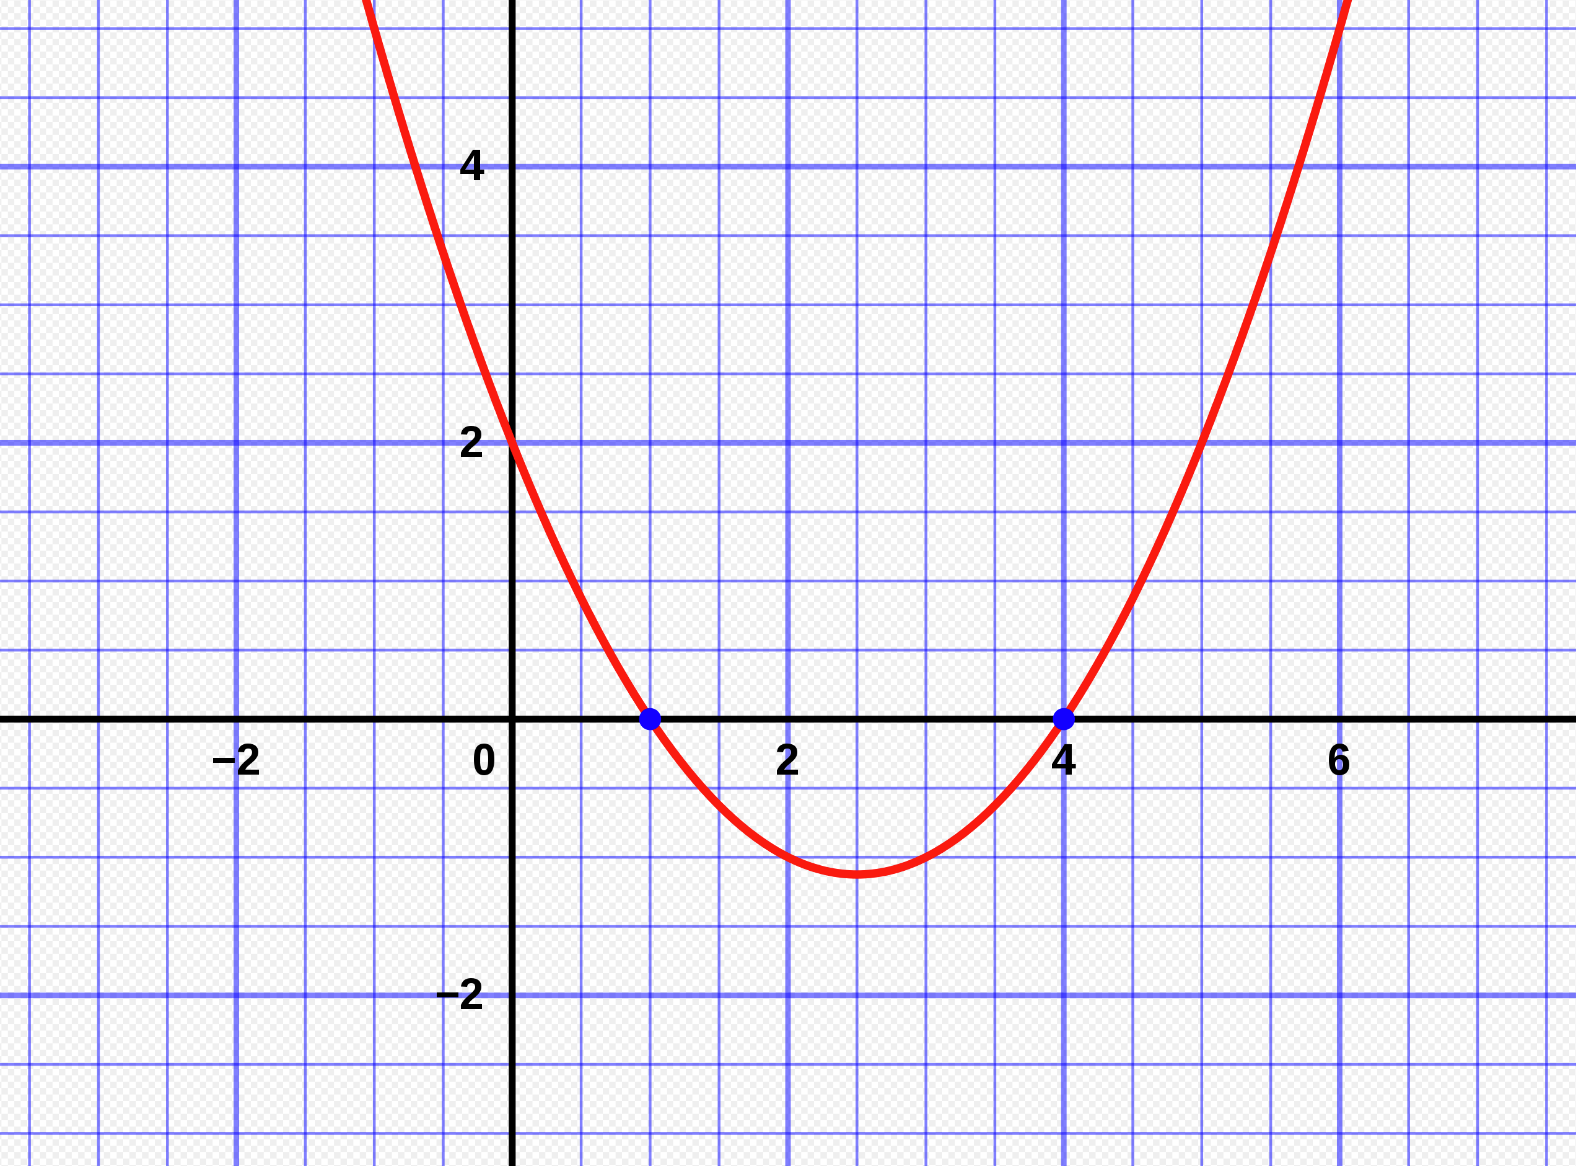
\includegraphics[scale=.15]{quad_equ.png} 

\begin{description}[labelindent=1cm]
	
	\item [\textbf{ \Large Overview}] \textbf{ \Large :}\\
	You will practice using strings in a Python program. The sequence operations will be used with strings, and several string methods are available for more advanced behaviors. 	
	\item[\textbf{\underline{System Requirements:}}] \hfill \vspace{0mm}

\begin{itemize}
	\item {\bf Computer}: A computer is required to complete this tutorial. Any OS should work.
	\item {\bf Python:} You can use the online Python compiler ( \href{https://www.online-python.com/online_python_compiler}{Online Python Compiler}  ) or a Python system of your choice.
\end{itemize}

	\item[\textbf{\underline{Background:}}] \hfill \vspace{0mm}
	
	\begin{description}

	 	\item [\textbf{String Parsing }] \textbf{ \Large :}\\   

            You are going to write a program to extract, or {\it parse}, the required information data from a given string. You can create your own string with your list from the previous tutorial or use the example provided. 
      
   \item[\textbf{\underline{Problem Statement:}}] \hfill \vspace{0mm}

	\begin{itemize}

		\item Given: A string or file containing the list of items. The string should be comma, newline, or space delimited.
		
		\item Complete: Generate a program to extract, or parse, the required information from the string. The extracted information should be printed to the screen.  

	\end{itemize}      

	\item[\textbf{\underline{Example Data to be Parsed:}}] \hfill \vspace{0mm}

	\begin{verbatim}
Name, ID, Price, Quantity
Motor, 103, $357.45, 2
Wheel, 78, $48.23, 4
LiDAR, 1089, $2500.00, 1
Computer, 99, $725.78, 1
Battery, 401, $501.01, 2
Battery Controller, 700, $58.99, 1
	\end{verbatim}
	\vspace*{10mm}
	(see tutorial5\_raw\_data.txt for data file)



	\end{description}


\newpage
\item[\textbf{\underline{Program Minimum Requirements:}}] \hfill \vspace{0mm}

The program should accomplish the following tasks. 

\begin{enumerate}
	
	\item Part 1 
		\begin{enumerate}

	      \item Initialize a single string named \lstinline{raw_data} containing all the data with comma, space, or newline deliniation. \\
	    
	      \item Extract the names of each of the items in \lstinline{raw_data}, and store all the names in a list called \lstinline{items}. \\

	      \item Extract the price of each item in \lstinline{raw_data}, and store the prices in a list called \lstinline{prices}. \\
	      
		\end{enumerate}	 

	\item Part 2
		\begin{enumerate}

	      \item Determine the most expensive item, and print the name and price to the screen.\\
	      
	      \item Determine the least expensive item, and print the name and price to the screen.\\

	      \item Determine the total cost of all the items combined. \\

		\end{enumerate}	

	\item Optional Advanced Features:
		\begin{itemize}
			
			\item Show the items with prices in order from least to greatest price.\\

			\item Show the items with prices in alphabetical order by name.\\	

			\item Modify the program to parse the string from a data file instead of a hardcoded literal.\\

			\item Modify the program to store the parsed data in a Python dictionary.\\		


		    
		\end{itemize}	

	\end{enumerate}
\newpage

\item[\textbf{\underline{Example Code:}}] \hfill \vspace{0mm}

	%\begin{minted}{cpp}
	\begin{lstlisting}

# Lists - GSET - Summer 2023 
	

	
	\end{lstlisting}
	%\end{minted}
		


	\item[\textbf{\underline{Part 3 - Testing:}}] \hfill \vspace{0mm}
	\begin{enumerate}
	
		\item Complete the Python code to the solve the problem described. \\\\
		
		\item Test your code with different inputs. Is the answer correct? How do you know? Are there certain inputs that do not work? \\\\
		
		\item Save your code with the download button or use copy and paste. You can view and edit the code in any text editor. Also, save a copy of the program output for your tutorial summary. \\\\

	\end{enumerate}

\newpage
\item[\textbf{\underline{Solution Code:}}] \hfill \vspace{0mm}

\begin{lstlisting}

COMING SOON
	
\end{lstlisting}

\item[\textbf{\underline{Tutorial Summary:}}] \hfill \vspace{3mm}\\ 
Write a brief summary of what you accomplished and what you struggled with the most. 

Include the following items in the summary:
\begin{itemize}

\item a copy of the output of your program
\item a description of what the program does and how to use it

\end{itemize}


\item[\textbf{\underline{Submission:}}] \hfill \vspace{3mm}\\ 
Use the appropriate assignment folder on ilearn to submit your program and summary. Submit the following items with your TNTech username in the filenames as shown below. \vspace{0mm}\\

\underline{Files for Tutorial 5 (TNTech Username : twhill21)}

\begin{itemize}

\item Tutorial Summary: \textbf{ twhill21\_summary5.txt}

\item Python Source Code: \textbf{ twhill21\_tutorial5.py}

\end{itemize}


\item[\textbf{\underline{Tutorial Complete:}}] \hfill \vspace{3mm}\\ 
	Congratulations, after completing {\it Tutorial 5 - The Shopping List}, you have learned the basics of Python! You are now ready to start learning about boolean logic and program flow. \\

\end{description}
\end{document}

